\documentclass[]{article}
\usepackage[UTF8]{ctex}
\usepackage[a4paper,left=10mm,right=10mm,bottom=10mm,top=10mm]{geometry}
\usepackage{graphicx}
\usepackage{float}
\usepackage{amsmath,amsfonts,amssymb,amsthm}
\usepackage{array,color}
%opening
\title{计算机科学中的数学基础--Exercise10}
\author{陈昱衡 521021910939}
\date{\today}

\begin{document}

\maketitle


\section*{Warmup6}
\begin{figure}[H]
    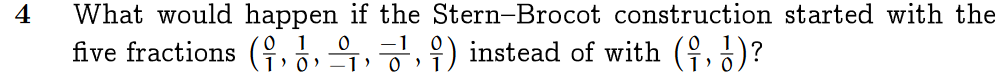
\includegraphics[scale = 0.6]{2023-03-16-10-44-42.png}
\end{figure}
用$({\frac{0}{1},\frac{1}{0},\frac{0}{-1},\frac{-1}{0},\frac{0}{1}})$替代$(\frac{0}{1},\frac{1}{0})$,我们发现,相邻的分数之间都会形成一棵类似于$(\frac{0}{1},\frac{1}{0})$所生成的树,只是分子和分母会有所差异.\par 
$(\frac{0}{1},\frac{1}{0})$之间形成的就是原先的树。\par 
$(\frac{1}{0},\frac{0}{-1})$之间形成的树的每一个节点上的分数的分母都会原先树的分母的相反数.且关于树的中轴线旋转。\par
$(\frac{0}{-1},\frac{-1}{0})$之间形成的树的每一个节点上的分数都与原先树相等,但是分子和分母都分别为相反数.\par 
$(\frac{-1}{0},\frac{0}{1})$之间形成的树的每一个节点的分数的分子都是原先树的相反数。\par
这样的话,生成的树中会有重复的数值,但是不会有重复的表示,可以刻画正有理数和负有理数。

\section*{Warmup7}
\begin{figure}[H]
    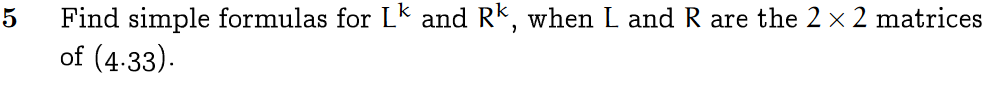
\includegraphics[scale = 0.6]{2023-03-16-10-46-00.png}
\end{figure}
$
L=
\begin{pmatrix}
    1 & 1 \\
    0 & 1 \\
\end{pmatrix}$
,我们进行矩阵分解,
L=$
\begin{pmatrix}
    1 & 0 \\
    0 & 1 \\
\end{pmatrix}
+ 
\begin{pmatrix}
    0 & 1\\
    0 & 0\\
\end{pmatrix}$
因此,
\begin{align}
    L^2&=
    \begin{pmatrix}
        1 & 1 \\
        0 & 1 \\
    \end{pmatrix}
    \times
    \left(
    \begin{pmatrix}
        1 & 0 \\
        0 & 1 \\
    \end{pmatrix}
    + 
    \begin{pmatrix}
        0 & 1\\
        0 & 0\\
    \end{pmatrix}
    \right)
    \\
    &=L+\begin{pmatrix}
        0 & 1\\
        0 & 0\\
    \end{pmatrix}
\end{align}
因此,使用数学归纳法,可以证明,
\begin{align}
    L^k &= L + \begin{pmatrix}
        0 & k-1\\
        0 & 0\\
    \end{pmatrix}\\
    &=\begin{pmatrix}
        1 & k\\
        0 & 1\\
    \end{pmatrix}
\end{align}
对矩阵R应用同样的过程,有
\begin{align}
    R^k &=
    \begin{pmatrix}
        1 & 0\\
        k & 1\\
    \end{pmatrix}
\end{align}

或者,借用书中4.5节的内容,可以得到,L和R可以理解为在Stern-Brocot树中向右或者向左遍历,因此,$L^k$可以理解为沿着根节点向左遍历k个节点,从Stern-Brocot树的图中可以读出,该节点表示的分数为$\frac{1}{k}$,
故,
\begin{align}
    M(\frac{1}{k})&= 
    \begin{pmatrix}
        n & kn^{'}+n\\
        m & km^{'}+m\\
    \end{pmatrix}
\end{align}
其中,由祖先分数$\frac{1}{1}$和$\frac{0}{1}$得到 n = 1,$n^{'}$=1,m=1,$m^{'}$=0.
故,
\begin{align}
    L^k &=
    \begin{pmatrix}
        1 & 0\\
        k & 1\\
    \end{pmatrix}
\end{align}
同理可得,
\begin{align}
    R^k &=
    \begin{pmatrix}
        1 & 0\\
        k & 1\\
    \end{pmatrix}
\end{align}

\section*{Warmup8}
\begin{figure}[H]
    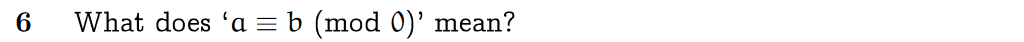
\includegraphics[scale = 0.6]{2023-03-16-10-46-48.png}
\end{figure}
根据mod的含义,可知,$a \equiv b \pmod{0}$的含义是a和b对0取模的结果相等。\par 
而a和b除以0的结果是$\inf$,余数分别为为a,b\par 
故,$a \equiv b \pmod{0}$的含义就是$a = b$,即在模意义下,当模数为 0 时,a 和 b 总是同余的。这是因为在模 0 意义下,任何两个整数都是等价的,因为它们之间的差值可以被 0 整除。\par 
由于在数学上没有定义“模 0”,因此这个等式在某些情况下可能没有意义。但是,在计算机科学中,这个等式可以用于说明两个整数在某些情况下是等价的。

\section*{Basics16}
\begin{figure}[H]
    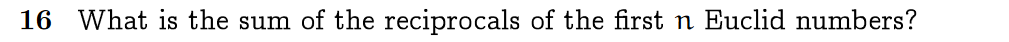
\includegraphics[scale = 0.6]{2023-03-16-10-47-05.png}
\end{figure}
首先,由前三项和,$\frac{1}{2}+\frac{1}{3}+\frac{1}{7} = \frac{41}{42}$,不妨猜想,欧拉数的前n项和为$\frac{e_{n+1} - 2}{e_{n+1} - 1}$,由此,我们可以从k = 3开始使用数学归纳法证明该结论.
\par 
\begin{align}
    \frac{1}{e_{1}} + \frac{1}{e_{2}} + \frac{1}{e_{3}} + \frac{1}{e_{4}} + \cdots + \frac{1}{e_{n}} &= \frac{e_{2} \times e_{3} \times \cdots \times e_{n} + e_{1} \times e_{3} \times \cdots \times e_{n} + \cdots + e_{2} \cdots e_{3} \cdots \times e_{n-1}}{e_{1} \times e_{2} \times \cdots \times  e_{n}}\\
    &= \frac{e_{2} \times e_{3} \times \cdots \times e_{n} + e_{1} \times e_{3} \times \cdots \times e_{n} + \cdots + e_{2} \cdots e_{3} \cdots \times e_{n-1}}{e_{n+1} - 1}\\
\end{align}
观察式子,发现分子比较难求,因此,可以对分子使用数学归纳法.
\par 
假定对于分子,前$k-1$项的和为$S_{k-1}$,可知由递推式
\begin{align}
    S_{k} &= e_{k} \times S_{k-1} + e_{1}\times e_{2} \times \cdots e_{k-1}\\
    &=e_{k} \times (e_{k} - 2) + e_{k} -1\\
    &=e_{k}^2 - e_{k} -1\\
    &=e_{k}(e_{k} - 1) - 1 \\
    &=e_{k} \times (e_{1} \times e_{2} \times \cdots \times e_{k-1}) -1\\
    &=e_{k} - 2
\end{align}
得证.\par 
因此,得到结论,前n项欧拉数的和为
\begin{align}
    \frac{e_{n+1} - 2}{e_{n+1} - 1} = 1-\frac{1}{e_{n+1} - 1}
\end{align}

\end{document}